\documentclass{article}

\usepackage{amsthm, amsfonts, amsmath, amssymb}
\allowdisplaybreaks[1]

\usepackage{graphicx}
\usepackage{fullpage}
\usepackage{float}
\usepackage{hyperref}

\newtheorem{lemma}{Lemma}
\newtheorem{theorem}{Theorem}
\newtheorem{corollary}{Corollary}
\newtheorem{conjecture}{Conjecture}
\newtheorem{definition}{Definition}

\setlength{\parindent}{0em}
\setlength{\parskip}{1em}

\renewcommand{\O}{\mathcal{O}}
\newcommand{\N}{\mathbb{N}}
\newcommand{\xor}{\oplus}
\renewcommand{\qedsymbol}{$\blacksquare$}

\begin{document}
	\title{A Generalized Approach to the Rank Deficiency of Certain Sized \textit{Lights Out} Boards}
	\author{William Boyles}
	\date{\today}
	\maketitle
	
	\section{Intro}
	In a previous document, we looked at boards of size $g(k) = 2^{k+1} + 2^{k-1} - 1$ for some natural number $k$.
	We can equivalently write $g(k) = 5\cdot2^{k-1} - 1$.
	We can thus generalize $g$ by allowing the leading coefficient to vary so we get
	\begin{equation*}
		g(b,k) = b\cdot2^{k-1} - 1.
	\end{equation*}
	We restrict $b$ to be odd as we want to maximize $k$.
	In the $b=5$ case, we were able to prove a general form of the Chebyshev polynomials for these board sizes and find the degree of their gcd.
	Thus, we were able to derive the rank deficiency of boards sized $g(5,k) \times g(5,k)$.
	We also conjectured that these boards represented exactly the highest rank deficiencies.
	In the next sections, we will investigate different values of $b$ and make conjectures about the corresponding Chebyshev polynomials and the rank deficiencies.
	
	First, we'll notice that every natural number can be represented in this form.
	\begin{lemma}
		Let $n \in \N$.
		Then $n$ can be represented in the form $b\cdot2^{k-1}$ where $b \in \N$ is odd and $k \in \N$.
	\end{lemma}
	\begin{proof}
		Since 2 is a prime, we can represent any natural number uniquely as $n = b\cdot2^{k-1}$, where $b$ is an odd natural and $k \in \N$.
	\end{proof}
	This proof also gives us a way to find $b$ and $k$ for any $n$: Simply divide by 2 as many times as possible. The number of times you divided is $k-1$, and the odd number you're left with is $b$.
	If we were to represent $n$ in binary, $b$ would be all the digits from the first 1 to the last 1, and $k-1$ would be the number of trailing 0's after the last 1.
	
	\newpage
	\section{When $b = 1$}
	If $b=1$, then $g(1,k) = 2^{k-1} - 1$.
	Below is a table of the Chebyshev polynomials for various values of $k$ and their gcd.
	
	\begin{table}[H]
		\renewcommand{\arraystretch}{1.5}
		\centering
		\begin{tabular}{|l||l|l|l|}
			\hline
			$k$ & $f(g(1,k),x)$ & $f(g(1,k),x+1)$ & $\gcd$  \\
			\hline\hline
			1 & $1$ & $1$ & $1$ \\
			\hline
			2 & $x$ & $x+1$ & $1$ \\
			\hline
			3 & $x^3$ & $x^3+x^2+x+1$ & $1$ \\
			\hline
			4 & $x^7$ & $x^7 + x^6 + \dots + x + 1$ & $1$ \\
			\hline
			5 & $x^{15}$ & $x^{15} + x^{14} + \dots + x + 1$ & $1$ \\
			\hline
			6 & $x^{31}$ & $x^{31} + x^{30} + \dots + x + 1$ & $1$ \\
			\hline
			7 & $x^{63}$ & $x^{63} + x^{62} + \dots + x + 1$ & $1$ \\
			\hline
			8 & $x^{127}$ & $x^{127} + x^{126} + \dots + x + 1$ & $1$ \\
			\hline  
		\end{tabular}
		\caption{Polynomials and their GCD for $b=1$}
	\end{table}
	Thus, we conjecture
	\begin{conjecture}
		Let $k \in \N$.
		Then the following are true:
		\begin{enumerate}
			\item
			\begin{equation*}
				f(g(1,k),x) = x^{g(1,k)}
			\end{equation*}
			\item
			\begin{equation*}
				f(g(1,k),x+1) = \sum_{n=0}^{g(1,k)}{x^n}
			\end{equation*}
			\item
			\begin{equation*}
				\gcd\left({f(g(1,k),x), f(g(1,k),x+1)}\right) = 1.
			\end{equation*}
		\end{enumerate}
	\end{conjecture}
	This conjecture implies that the nullity of all boards of size $g(1,k) \times g(1,k)$ is $0$.
	This is consistent with computer results.
	
	Notice that statement 1 implies statement 2 because
	\begin{align*}
		f(g(1,k),x) &= x^{g(1,k)} \\
		f(g(1,k),x+1) &= (x+1)^{g(1,k)} \\
			&= \frac{(x+1)^{2^{k-1}}}{x+1} \\
			&\equiv \frac{x^{2^{k-1}}+1}{x+1} \\
			&\equiv \frac{1-x^{2^{k-1}}}{1-x} \\
			&= 1 + \dots + x^{g(1,k)} \\
			&= \sum_{n=0}^{g(1,k)}{x^n}.
	\end{align*}
	
	It's not too difficult to see in this case that statements 1 and 2 together imply statement 3.
	Thus, we only need to prove statement 1 true to prove the conjecture.
	
	\newpage
	\section{When $b = 3$}
	If $b=3$, then $g(3,k) = 3\cdot2^{k-1} - 1$.
	Below is a table of the Chebyshev polynomials for various values of $k$ and their gcd.
	
	\begin{table}[H]
		\renewcommand{\arraystretch}{1.5}
		\centering
		\begin{tabular}{|l||l|l|l|}
			\hline
			$k$ & $f(g(3,k),x)$ & $f(g(3,k),x+1)$ & $\gcd$  \\
			\hline\hline
			1 & $x^2 + 1$ & $x^2$ & $1$ \\
			\hline
			2 & $x^5 + x$ & $x^5 + x^4$ & $x^2 + x$ \\
			\hline
			3 & $x^{11} + x^3$ & $x^{11} + x^{10} + x^9 + x^8$ & $x^6 + x^5 + x^4 + x^3$ \\
			\hline
			4 & $x^{23} + x^{7}$ & $x^{23} + \dots + x^{16}$ & $x^{14} + \dots + x^7$ \\
			\hline
			5 & $x^{47} + x^{15}$ & $x^{47} + \dots + x^{32}$ & $x^{30} + \dots + x^{15}$ \\
			\hline
			6 & $x^{95} + x^{31}$ & $x^{95} + \dots + x^{64}$ & $x^{62} + \dots + x^{31}$ \\
			\hline
			7 & $x^{191} + x^{63}$ & $x^{191} + \dots + x^{128}$ & $x^{126} + \dots + x^{63}$ \\
			\hline
			8 & $x^{383} + x^{127}$ & $x^{383} + \dots + x^{256}$ & $x^{254} + \dots + x^{127}$ \\
			\hline  
		\end{tabular}
		\caption{Polynomials and their GCD for $b=3$}
	\end{table}
	Thus, we conjecture
	\begin{conjecture}
		Let $k \in \N$.
		Then the following are true:
		\begin{enumerate}
			\item
			\begin{equation*}
				f(g(3,k),x) = x^{g(3,k)} + x^{g(1,k)}.
			\end{equation*}
			\item
			\begin{equation*}
				f(g(3,k),x+1) = \sum_{n=2^k}^{g(3,k)}{x^n} = x^{2^k}\sum_{n=0}^{g(1,k)}{x^n}.
			\end{equation*}
			\item
			\begin{equation*}
				\gcd\left({f(g(1,k),x), f(g(1,k),x+1)}\right) = \sum_{n=g(1,k)}^{2g(1,k)}{x^n} = x^{g(1,k)}\sum_{n=0}^{g(1,k)}{x^n}.
			\end{equation*}
		\end{enumerate}
	\end{conjecture}
	This conjecture implies that the nullity of all boards of size $g(3,k) \times g(3,k)$ is $2g(1,k)$.
	This is consistent with computer results.
	
	Notice that statement 1 implies statement 2 because
	\begin{align*}
		f(g(3,k),x) &= x^{g(3,k)} + x^{g(1,k)} \\
		f(g(3,k),x+1) &= (x+1)^{g(3,k)} + (x+1)^{g(1,k)} \\
		&= \frac{1}{x+1}\left((x+1)^{3\cdot2^{k-1}} + (x+1)^{2^{k-1}}\right) \\
		&= \frac{(x+1)^{2^{k-1}}}{x+1}\left((x+1)^{2\cdot2^{k-1}}+1\right) \\
		&\equiv \frac{x^{2^{k-1}}+1}{x+1}\left(x^{2\cdot2^{k-1}}+1+1\right) \\
		&\equiv \frac{1-x^{2^{k-1}}}{1-x}x^{2\cdot2^{k-1}} \\
		&= \left(1+\dots+x^{2^{k-1}-1}\right)x^{2\cdot2^{k-1}} \\
		&= x^{2\cdot2^{k-1}} + \dots + x^{3\cdot2^{k-1}-1} \\
		&= x^{2^k}\sum_{n=0}^{g(1,k)}{x^n}.
	\end{align*}

	\newpage
	\section{When $b = 5$}
	We already covered this specific case in another work.
	The main result is that the degree of the GCD of the polynomials is $2^{k+1}$.
	However, for completeness, we'll list out some values in a table and state the conjecture.
	
	\begin{table}[H]
		\renewcommand{\arraystretch}{1.5}
		\centering
		\begin{tabular}{|l||l|l|l|}
			\hline
			$k$ & $f(g(5,k),x)$ & $f(g(5,k),x+1)$ & $\gcd$  \\
			\hline\hline
			1 & $x^4 + x^2 + 1$ & $x^4 + x^2 + 1$ & $x^4 + x^2 + 1$ \\
			\hline
			2 & $x^9 + x^5 + x$ & $\left(x^9 + x^8\right) + \left(x^5 + x^4\right) + \left(x + 1\right)$ & $x^8 + x^4 + 1$ \\
			\hline
			3 & $x^{19} + x^{11} + x^3$ & $\left(x^{19}+\dots+x^{16}\right)+\left(x^{11}+\dots+x^{8}\right)+\left(x^{3}+\dots+1\right)$ & $x^{16} + x^8 + 1$ \\
			\hline
			4 & $x^{39} + x^{23} + x^{7}$ & $\left(x^{39}+\dots+x^{32}\right)+\left(x^{23}+\dots+x^{16}\right)+\left(x^{7}+\dots+1\right)$ & $x^{32} + x^{16} + 1$\\
			\hline
			5 & $x^{79} + x^{47} + x^{15}$ & $\left(x^{79}+\dots+x^{64}\right)+\left(x^{47}+\dots+x^{32}\right)+\left(x^{15}+\dots+1\right)$ & $x^{64} + x^{32} + 1$ \\
			\hline
			6 & $x^{159} + x^{95} + x^{31}$ & $\left(x^{159}+\dots+x^{128}\right)+\left(x^{95}+\dots+x^{64}\right)+\left(x^{31}+\dots+1\right)$ & $x^{128} + x^{64} + 1$\\
			\hline
			7 & $x^{319} + x^{191} + x^{63}$ & $\left(x^{319}+\dots+x^{256}\right)+\left(x^{191}+\dots+x^{128}\right)+\left(x^{63}+\dots+1\right)$ & $x^{256} + x^{128} + 1$ \\
			\hline
			8 & $x^{639} + x^{383} + x^{127}$ & $\left(x^{639}+\dots+x^{512}\right)+\left(x^{383}+\dots+x^{256}\right)+\left(x^{127}+\dots+1\right)$ & $x^{512} + x^{256} + 1$ \\
			\hline
		\end{tabular}
		\caption{Polynomials and their GCD for $b=5$}
	\end{table}

	Thus, we've conjecture (and subsequently proved)
	\begin{lemma}
		Let $k \in \N$.
		Then the following are true:
		\begin{enumerate}
			\item
			\begin{equation*}
				f(g(5,k),x) = x^{g(5,k)} + x^{g(3,k)} + x^{g(1,k)}.
			\end{equation*}
			\item
			\begin{equation*}
				f(g(5,k),x+1) = \sum_{m\in\{1,3,5\}}{\sum_{n=0}^{g(1,k)}{x^{g(m,k)-n}}}.
			\end{equation*}
			\item
			\begin{equation*}
				\gcd\left(f(g(5,k),x), f(g(5,k),x+1)\right) = \sum_{m\in\{1,3,5\}}{x^{g(m,k)-g(1,k)}}.
			\end{equation*}
		\end{enumerate}
	\end{lemma}
	This lemma implies that the nullity of all boards of size $g(5,k) \times g(5,k)$ is $2^{k+1}$.
	This is consistent (as it must be if proven true) with computer result.
	
	\newpage
	\section{When $b = 7$}
	If $b=7$, then $g(7,k) = 7\cdot2^{k-1}-1$.
	Below is a table of the Chebyshev polynomials for various values of $k$ and their gcd.
	
	\begin{table}[H]
		\renewcommand{\arraystretch}{1.5}
		\centering
		\begin{tabular}{|l||l|l|l|}
			\hline
			$k$ & $f(g(7,k),x)$ & $f(g(7,k),x+1)$ & $\gcd$  \\
			\hline\hline
			1 & $x^6 + x^4 + 1$ & $x^6 + x^2 + 1$ & $1$ \\
			\hline
			2 & $x^{13} + x^9 + x$ & $\left(x^{13} + x^{12}\right) + \left(x^{5} + x^{4}\right) + \left(x + 1\right)$ & $1$ \\
			\hline
			3 & $x^{27} + x^{19} + x^3$ & $\left(x^{27} + \dots + x^{24}\right) + \left(x^{11} + \dots + x^8\right) + \left(x^3 \dots + 1\right)$ & $1$ \\
			\hline
			4 & $x^{55} + x^{39} + x^7$ & $\left(x^{55}+\dots+x^{48}\right)+\left(x^{23}+\dots+x^{16}\right)+\left(x^7+\dots+1\right)$ & $1$ \\
			\hline 
			5 & $x^{111} + x^{79} + x^{15}$ & $\left(x^{111}+\dots+x^{96}\right)+\left(x^{57}+\dots+x^{32}\right)+\left(x^{15}+\dots+1\right)$ & $1$ \\
			\hline
			6 & $x^{223} + x^{159} + x^{31}$ & $\left(x^{223}+\dots+x^{192}\right)+\left(x^{115}+\dots+x^{64}\right)+\left(x^{31}+\dots+1\right)$ & $1$ \\
			\hline
			7 & $x^{447} + x^{319} + x^{63}$ & $\left(x^{447}+\dots+x^{384}\right)+\left(x^{231}+\dots+x^{128}\right)+\left(x^{63}+\dots+1\right)$ & $1$ \\
			\hline
			8 & $x^{895} + x^{639} + x^{127}$ & $\left(x^{895}+\dots+x^{768}\right)+\left(x^{463}+\dots+x^{256}\right)+\left(x^{127}+\dots+1\right)$ & $1$ \\
			\hline
		\end{tabular}
		\caption{Polynomials and their GCD for $b=7$}
	\end{table}

	Thus, we conjecture
	\begin{conjecture}
		Let $k \in \N$.
		Then the following are true:
		\begin{enumerate}
			\item
			\begin{equation*}
				f(g(7,k),x) = x^{g(7,k)} + x^{g(5,k)} + x^{g(1,k)}.
			\end{equation*}
			\item
			\begin{equation*}
				f(g(7,k),x+1) = \sum_{m\in\{1,3,7\}}{\sum_{n=0}^{g(1,k)}{x^{g(m,k)-n}}}
			\end{equation*}
			\item
			\begin{equation*}
				\gcd\left(f(g(7,k),x),f(g(7,k),x+1)\right) = 1.
			\end{equation*}
		\end{enumerate}
	\end{conjecture}
	This conjecture implies that the nullity of all boards of size $g(7,k) \times g(7,k)$ is 0.
	This is consistent with computer results.
	
	Notice that statement 1 implies statement 2 because
	\begin{align*}
		f(g(7,k),x) &= x^{g(7,k)} + x^{g(5,k)} + x^{g(1,k)} \\
		f(g(7,k),x+1) &= (x+1)^{g(7,k)} + (x+1)^{g(5,k)} + (x+1)^{g(1,k)} \\
		%&= (x+1)^{7\cdot2^{k-1}-1} + (x+1)^{5\cdot2^{k-1}-1} + (x+1)^{2^{k-1}-1} \\
		&= \frac{1}{x+1} \left((x+1)^{7\cdot2^{k-1}} + (x+1)^{5\cdot2^{k-1}} + (x+1)^{2^{k-1}}\right) \\
		&= \frac{(x+1)^{2^{k-1}}}{x+1}\left((x+1)^{4\cdot2^{k-1}}(x+1)^{2\cdot2^{k-1}}+(x+1)^{4\cdot2^{k-1}}+1\right) \\
		&\equiv \frac{x^{2^{k-1}}+1}{x+1}\left(\left(x^{4\cdot2^{k-1}}+1\right)\left(x^{2\cdot2^{k-1}}+1\right)+\left(x^{4\cdot2^{k-1}}+1\right)+1\right) \\
		&\equiv \frac{1-x^{2^{k-1}}}{1-x}\left(x^{6\cdot2^{k-1}}+x^{4\cdot2^{k-1}}+x^{2\cdot2^{k-1}}+1+x^{4\cdot2^{k-1}}+1+1\right) \\
		&\equiv \frac{1-x^{2^{k-1}}}{1-x}\left(x^{6\cdot2^{k-1}}+x^{2\cdot2^{k-1}}+1\right) \\
		&= \left(1+\dots+x^{2^{k-1}-1}\right)\left(x^{6\cdot2^{k-1}}+x^{2\cdot2^{k-1}}+1\right) \\
		&= \left(x^{6\cdot2^{k-1}}+\dots+x^{7\cdot2^{k-1}-1}\right) + \left(x^{2\cdot2^{k-1}}+\dots+x^{3\cdot2^{k-1}-1}\right) + \left(1+\dots+x^{2^{k-1}-1}\right) \\
		&= \sum_{m\in\{1,3,7\}}{\sum_{n=0}^{g(1,k)}{x^{g(m,k)-n}}}.
	\end{align*}
	
	\newpage
	\section{When $b = 9$}
	If $b=9$, then $g(9,k) = 9\cdot2^{k-1} - 1$.
	Below is a table of Chebyshev polynomials for various values of $k$ and their GCD.
	
	\begin{table}[H]
		\renewcommand{\arraystretch}{1.5}
		\centering
		\begin{tabular}{|l||l|l|l|}
			\hline
			$k$ & $f(g(9,k),x)$ & $f(g(9,k),x+1)$ & $\gcd$ \\
			\hline \hline
			1 & $x^8 + x^6 + x^4 + 1$ & $x^8 + x^6 + x^2$ & $1$ \\
			\hline
			2 & $x^{17} + x^{13} + x^{9} + x$ & $\left(x^{17} + x^{16}\right) + \left(x^{13} + x^{12}\right) + \left(x^{5} + x^{4}\right)$ & $x^2 + x$ \\
			\hline
			3 & $x^{35} + x^{27} + x^{19} + x^{3}$ & $\left(x^{35}+\dots+x^{32}\right)+\left(x^{27}+\dots+x^{24}\right)+\left(x^{11}+\dots+x^8\right)$& $x^6 + x^5 + x^4 + x^3$ \\
			\hline
			4 & $x^{71} + x^{55} + x^{39} + x^{7}$ & $\left(x^{71}+\dots+x^{64}\right)+\left(x^{55}+\dots+x^{48}\right)+\left(x^{23}+\dots+x^{16}\right)$ & $x^{14} + \dots + x^7$ \\
			\hline
			5 & $x^{143} + x^{111} + x^{79} + x^{15}$ & $\left(x^{143}+\dots+x^{128}\right)+\left(x^{111}+\dots+x^{96}\right)+\left(x^{57}+\dots+x^{32}\right)$ & $x^{30} + \dots + x^{15}$ \\
			\hline
			6 & $x^{287} + x^{223} + x^{159} + x^{31}$ & $\left(x^{287}+\dots+x^{256}\right)+\left(x^{223}+\dots+x^{192}\right)+\left(x^{115}+\dots+x^{64}\right)$ & $x^{62} + \dots + x^{31}$ \\
			\hline
			7 & $x^{757} + x^{447} + x^{319} + x^{63}$ & $\left(x^{757}+\dots+x^{512}\right)+\left(x^{447}+\dots+x^{384}\right)+\left(x^{231}+\dots+x^{128}\right)$ & $x^{126} + \dots + x^{63}$ \\
			\hline
			8 & $x^{1515} + x^{895} + x^{639} + x^{127}$ & $\left(x^{1515}+\dots+x^{1024}\right)+\left(x^{895}+\dots+x^{768}\right)+\left(x^{463}+\dots+x^{256}\right)$ & $x^{254} + \dots + x^{127}$ \\
			\hline
		\end{tabular}
		\caption{Polynomials and their GCD for $b=9$}
	\end{table}

	Thus, we conjecture
	\begin{conjecture}
		Let $k \in \N$.
		Then the following are true:
		\begin{enumerate}
			\item
			\begin{equation*}
				f(g(9,k),x) = x^{g(9,k)} + x^{g(7,k)} + x^{g(5,k)} + x^{g(1,k)}.
			\end{equation*}
			\item
			\begin{equation*}
				f(g(9,k),x+1) = \sum_{m\in\{3,7,9\}}{\sum_{n=0}^{g(1,k)}{x^{g(m,k)-n}}}.
			\end{equation*}
			\item
			\begin{equation*}
				\gcd\left(f(g(9,k),x),f(g(9,k),x+1)\right) = x^{g(1,k)}\sum_{n=0}^{g(1,k)}{x^n}.
			\end{equation*}
		\end{enumerate}
	\end{conjecture}
	This conjecture implies that the nullity of all boards of size $g(9,k) \times g(9,k)$ is $2g(1,k)$.
	This is consistent with computer results.
	
	Notice that statement 1 implies statement 2 because
	\begin{align*}
		f(g(9.k),x) &= x^{g(9,k)} + x^{g(7,k)} + x^{g(5,k)} + x^{g(1,k)} \\
		f(g(9,k),x+1) &= (x+1)^{g(9,k)} + (x+1)^{g(7,k)} + (x+1)^{g(5,k)} + (x+1)^{g(1,k)} \\
		&= \frac{1}{x+1}\left((x+1)^{9\cdot2^{k-1}} + (x+1)^{7\cdot2^{k-1}} + (x+1)^{5\cdot2^{k-1}} + (x+1)^{2^{k-1}}\right) \\
		&= \frac{(x+1)^{2^{k-1}}}{x+1}\left((x+1)^{8\cdot2^{k-1}} + (x+1)^{4\cdot2^{k-1}}(x+1)^{2\cdot2^{k-1}} + (x+1)^{4\cdot2^{k-1}} + 1\right) \\
		&\equiv \frac{x^{2^{k-1}}+1}{x+1}\left(\left(x^{8\cdot2^{k-1}}+1\right) + \left(x^{4\cdot2^{k-1}}+1\right)\left(x^{2\cdot2^{k-1}}+1\right) + \left(x^{4\cdot2^{k-1}}+1\right) + 1\right) \\
		&\equiv \frac{1-x^{2^{k-1}}}{1-x}\left(x^{8\cdot2^{k-1}} + 1 + x^{6\cdot2^{k-1}} + x^{4\cdot2^{k-1}} + x^{2\cdot2^{k-1}} + 1 + x^{4\cdot2^{k-1}} + 1 + 1\right) \\
		&\equiv \frac{1-x^{2^{k-1}}}{1-x}\left(x^{8\cdot2^{k-1}}+x^{6\cdot2^{k-1}}+x^{2\cdot2^{k-1}}\right) \\
		&= \left(1+\dots+x^{2^{k-1}-1}\right)\left(x^{8\cdot2^{k-1}}+x^{6\cdot2^{k-1}}+x^{2\cdot2^{k-1}}\right) \\
		&= \left(x^{8\cdot2^{k-1}}+\dots+x^{9\cdot2^{k-1}-1}\right) + \left(x^{6\cdot2^{k-1}}+\dots+x^{7\cdot2^{k-1}-1}\right) + \left(x^{2\cdot2^{k-1}}+\dots+x^{3\cdot2^{k-1}-1}\right) \\
		&= \sum_{m\in\{3,7,9\}}{\sum_{n=0}^{g(1,k)}{x^{g(m,k)-n}}}.
	\end{align*}
	Also, notice that we have the same conjectured GCD result here as for $b=3$.
	In fact, we can somewhat ``see'' the parts from $b=3$ in our table.
	The last grouping of terms in the $f(g(9,k),x+1)$ column are exactly the same terms as in the entire $f(g(3,k),x+1)$ column.

	\newpage
	\section{Meta-Results}
	Now that we've seen many examples of how these polynomials and their GCDs because for various values of $b$ and $k$, we'll prove some results about their behavior as $k$ varies.
	
	\begin{lemma}
		Let
		\begin{equation*}
			f(g(b,k),x) = x^{n_1} + x^{n_2} + \dots + x^{n_m}.
		\end{equation*}
		Then
		\begin{equation*}
			f(g(b,k+1),x) = x^{2n_1 + 1} + x^{2n_2 + 1} + \dots + x^{2n_m + 1}.
		\end{equation*}
	\end{lemma}
	\begin{proof}
		Consider how we calculate $f(n,x)$ in our code.
		We say
		\begin{align*}
			l(n) &= 2^{\lceil \log_2{(n+1)} \rceil} - 1 \\
			s(n) &= 2(l(n) - n).
		\end{align*}
		For $f(g(b,k),x)$,
		\begin{align*}
			l(g(b,k)) &= 2^{\lceil \log_2{\left(b\cdot2^{k-1}\right)} \rceil} - 1 \\
			&= 2^{\lceil \log_2{\left(2^{k-1}\right)}+ \log_2{(b)} \rceil} - 1 \\
			&= 2^{\lceil k-1 + \log_2{(b)} \rceil} - 1 \\
			&= 2^{k + \lfloor \log_2{(b)} \rfloor} - 1. \\
			s(g(b,k)) &= 2\left(2^{k+\lfloor\log_2{(b)}\rfloor} - 1 - b\cdot2^{k-1} + 1\right) \\
			&= 2\left(2^{k + \lfloor \log_2{(b)} \rfloor} - b\cdot2^{k-1}\right) \\
			&= 2^{k+1+\lfloor\log_2{(b)}\rfloor} - b\cdot2^{k} \\
			&= 2^{k}\left(2^{\lceil \log_2{(b)}\rceil} - b\right).
		\end{align*}
		To calculate to polynomial as a list of coefficients,
		\begin{equation*}
			\left[\binom{s(n) + 2i}{s(n) + i} \mod 2 \texttt{ for i in range(n+1)} \right],
		\end{equation*}
		where
		\begin{equation*}
			\binom{n}{m} \mod 2 = \begin{cases}
				0 & \texttt{((n-m) \& m) != 0} \\
				1 & \text{otherwise}
			\end{cases}.
		\end{equation*}
		For $f(g(b,k),x)$,
		\begin{align*}
			\binom{s(g(b,k))+2i}{s(g(b,k))+i} \mod 2 &= \binom{2^{k}\left(2^{\lceil \log_2{(b)}\rceil} - b\right) + 2i}{2^{k}\left(2^{\lceil \log_2{(b)}\rceil} - b\right) + i} \mod 2 \\
			&= \begin{cases}
				0 & \texttt{i \& }\left(2^{k}\left(2^{\lceil \log_2{(b)}\rceil} - b\right) \texttt{ + i}\right)\texttt{ != 0} \\
				1 & \text{otherwise}
			\end{cases}.
		\end{align*}
		Imagine that for some $i$, $b$, and $k$ that
		\begin{align*}
			\binom{s(g(b,k)) + 2i}{s(g(b,k)) + i} \mod 2 &= 0 \\
			\texttt{i \& }\left(2^{k}\left(2^{\lceil\log_2{(b)}\rceil} - b\right)\texttt{+ i}\right) &\neq 0.
		\end{align*}
		Then
		\begin{align*}
			\texttt{2i \& }2\left(2^{k}\left(2^{\lceil\log_2{(b)}\rceil} - b\right)\texttt{+ i}\right) &\neq 0.
		\end{align*}
		Recall that our list of coefficients represents polynomials with the highest degree as the first term (i.e. index 0).
		Thus, the sum of the index and the degree for $f(n,x)$ is always equal to $n$.
		So, for $f(g(b,k),x)$,
		\begin{align*}
			\deg_{i,k} + i &= g(b,k) \\
			\deg_{i,k} &= g(b,k) - i
		\end{align*}
		where $\deg_{i,k}$ is the corresponding degree of the coefficient at index $i$ in our representation of $f(g(b,k))$.
		So, for $f(g(b,k+1),x)$,
		\begin{align*}
			\deg_{2i,k+1} + 2i &= g(b,k+1) \\
			\deg_{2i,k+1} &= g(b,k+1) - 2i \\
			&= b\cdot2^{k} - 1 - 2i \\
			&= 2\left(b\cdot2^{k-1} - 1 - i\right) + 1 \\
			&= 2\left(g(b,k) - i\right) + 1 \\
			&= 2\deg_{i,k} + 1.
		\end{align*}
		So, we see that
		\begin{equation*}
			\binom{s(g(b,k)) + 2i}{s(g(b,k)) + i} \mod 2 = 0 \implies \binom{s(g(b,k+1)) + 4i}{s(g(b,k+1)) + 2i} \mod 2 = 0.
		\end{equation*}
		The same logic applies to show that both sides get the same result if the parity is odd. Thus,
		\begin{equation*}
			\binom{s(g(b,k)) + 2i}{s(g(b,k)) + i} \equiv \binom{s(g(b,k+1)) + 4i}{s(g(b,k+1)) + 2i} \mod 2.
		\end{equation*}
		Now we just need to consider odd indices $i$ in $f(g(b,k),x)$.
		Recall that for any index $i$,
		\begin{equation*}
			\binom{s(g(b,k)) + 2i}{s(g(b,k)) + i} \mod 2 =\begin{cases}
				0 & \texttt{i \& }\left(s(g(b,k)) + i\right) \neq 0 \\
				1 & \text{otherwise}
			\end{cases}.
		\end{equation*}
		Since $s(g(b,k)) = 2^k\left(2^{\lceil \log_2{(b)} \rceil} - b\right)$, and $k \in \N$,
		$s(g(b,k))$ is always even.
		Thus for odd $i$, both $i$ and $s(g(b,k)) + i$ will be odd.
		Therefore, the result of their bitwise AND (i.e. \texttt{\&}) will be non-zero.
		So, all odd indices $i$ in $f(g(b,k+1))$ will be 0 in our polynomial representation.
	\end{proof}
	This implies that if we know the exponents of $f(g(b,1),x)$, we can iteratively calculate them for any $f(g(b,k),x)$.
	
	\begin{corollary}
		For all $k \in \N$, $x^{g(1,k)}$ divides $f(g(b,k),x)$.
	\end{corollary}
	\begin{proof}
		By induction on $k$.
		Notice that for $k=1$, $g(1,1) = 1\cdot2^{1-1} - 1 = 0$, and $x^0 = 1$ trivially divides everything.
		Assume for some $k \in \N$ that $x^{g(1,k)}$ divides $f(g(b,k),x)$.
		That is,
		\begin{equation*}
			f(g(b,k),x) = x^{a_1} + x^{a_2} + \dots + x^{a_n},
		\end{equation*}
		where $a_1 > a_2 > \dots > a_n \geq g(1,k)$.
		Then
		\begin{equation*}
			f(g(b,k+1),x) = x^{2a_1 + 1} + x^{2a_2 + 1} + \dots + x^{2a_n + 1}.
		\end{equation*} 
		So, $2a_1 + 1 > 2a_2 + 1 > \dots > 2a_n + 1 \geq 2g(1,k)+1 = g(1,k+1),$ as desired.
	\end{proof}
	
	\begin{corollary}\label{fx-iterative-col}
		The following identity holds:
		\begin{equation*}
			f(g(b,k+1),x) = x\left(f(g(b,k),x)\right)^2.
		\end{equation*}
	\end{corollary}
	\begin{proof}
		Let
		\begin{equation*}
			f(g(b,k),x) = x^{a_1} + x^{a_2} + \dots + x^{a_n},
		\end{equation*}
		where $a_1 > a_2 > \dots > a_n \geq 0$.
		Then
		\begin{align*}
			f(g(b,k+1),x) &= x^{2a_1 + 1} + x^{2a_2 + 1} + \dots + x^{2a_n+1} \\
			&= x\left(x^{2a_1} + x^{2a_2} + \dots + x^{2a_n}\right) \\
			&=\equiv x\left(x^{a_1} + x^{a_2} + \dots + x^{a_n}\right)^2 \\
			&= x\left(f(g(b,k),x)\right)^2,
		\end{align*}
		as desired.
	\end{proof}
	
	\begin{corollary}\label{fx1-iterative-col}
		The following identity holds:
		\begin{equation*}
			f(g(b,k+1),x+1) = (x+1)\left(f(g(b,k),x+1)\right)^2.
		\end{equation*}
	\end{corollary}
	
	We can also establish a corollary that seems to have an interesting connection to another part of mathematics.
	\begin{corollary}
		For a fixed value of $b$, the number of non-zero terms in $f(g(b,k),x)$ is the same for all $k$.
	\end{corollary}
	Below is a table of various values of $b$ and the number of non-zero terms in $f(g(b,k),x)$.
	
	\begin{table}[H]
		\centering
		\begin{tabular}{|l||l|}
			\hline
			$b$ & Number of Non-Zero Terms in $f(g(b,k),x)$ \\
			\hline\hline
			1 & 1 \\
			\hline
			3 & 2 \\
			\hline
			5 & 3 \\
			\hline
			7 & 3 \\
			\hline
			9 & 4 \\
			\hline
			11 & 5 \\
			\hline
			13 & 5 \\
			\hline
			15 & 4 \\
			\hline
			17 & 5 \\
			\hline
			19 & 7 \\
			\hline
			21 & 8 \\
			\hline
			23 & 7 \\
			\hline
			25 & 7 \\
			\hline
			27 & 8 \\
			\hline
			29 & 7 \\
			\hline
		\end{tabular}
		\caption{Number of non-zero terms in $f(g(b,k),x)$.}
	\end{table}
	
	Putting this sequence into the OEIS, we see that it matches with \href{https://oeis.org/A007306}{A007306}, which are the denominators of Farey tree fractions, which is pictured below.
	We can see that the sequence is simply the denominators of the tree read level by level, left to right.
	
	\begin{figure}[H]
		\centering
		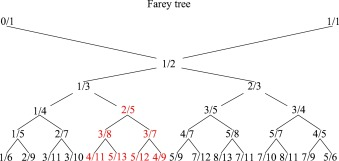
\includegraphics[width=0.8\textwidth]{farey_tree.jpg}
		\caption{Farey Tree in range [0,1]. Also known as Stern-Brocot Tree.}
	\end{figure}

	\newpage
	\begin{lemma}
		Choose any $b \in \N$ odd and $k \in \N$.
		Let
		\begin{equation*}
			f(g(b,k),x+1) = x^{n_1} + x^{n_2} + \dots + x^{n_m}.
		\end{equation*}
		Then
		\begin{equation*}
			f(g(b,k+1),x+1) = x^{2n_1 + 1} + x^{2n_1} + x^{2n_2 + 1} + x^{2n_2} + \dots + x^{2n_m + 1} + x^{2n_m}.
		\end{equation*}
	\end{lemma}
	\begin{proof}
		Notice that if
		\begin{equation*}
			f(g(b,k),x) = x^{a_1} + x^{a_2} + \dots + x^{a_m},
		\end{equation*}
		then
		\begin{equation*}
			f(g(b,k),x+1) = (x+1)^{a_1} + (x+1)^{a_2} + \dots + (x+1)^{a_m}.
		\end{equation*}
		Assume that
		\begin{equation*}
			f(g(b,k),x+1) = x^{b_1} + x^{b_2} + \dots + x^{b_n}.
		\end{equation*}
		Then
		\begin{align*}
			f(g(b,k),x+1) &= (x+1)^{a_1} + (x+1)^{a_2} + \dots + (x+1)^{a_m} \\
			f(g(b,k+1),x+1) &= (x+1)^{2a_1 + 1} + (x+1)^{2a_2 + 1} + \dots + (x+1)^{2a_m + 1} \\
			&= (x+1)\left((x+1)^{2a_1} + (x+1)^{2a_2} + \dots + (x+1)^{2a_m}\right) \\
			&\equiv (x+1)\left((x+1)^{a_1} + (x+1)^{a_2} + \dots + (x+1)^{a_m}\right)^2 \\
			&= (x+1)\left(x^{b_1} + x^{b_2} + \dots + x^{b_n}\right)^2 \\
			&\equiv (x+1)\left(x^{2b_1} + x^{2b_2} + \dots + x^{2b_n}\right) \\
			&= x^{2b_1 + 1} + x^{2b_1} + x^{2b_2 + 1} + x^{2b_2} + \dots + x^{2b_n + 1} + x^{2b_n},
		\end{align*}
		as desired.
	\end{proof}
	This implies that if we know the exponents of $f(g(b,1),x+1)$, we can iteratively calculate them for any $f(g(b,k),x+1)$. \\
	
	Like previously, we can establish a corollary about the number of non-zero terms.
	\begin{corollary}
		Choose any $b \in \N$ odd and $k \in \N$.
		Then the number of non-zero terms in $f(g(b,k),x+1)$ is $2^{k-1}$ times as many non-zero terms as in $f(g(b,1),x+1)$.
	\end{corollary}
	Notice that means we can write the number of non-zero terms in $f(g(b,k),x+1)$ as $g(b',k)$, where $b'$ is the number of non-zero terms in $f(g(b,1),x+1)$.
	Below is a table of various values of $b$ and the number of non-zero terms in $f(g(b,1),x+1)$.
	
	\begin{table}[H]
		\centering
		\begin{tabular}{|l||l|}
			\hline
			$b$ & Non-Zero Terms in $f(g(b,1),x+1)$ \\
			\hline\hline
			1 & 1 \\
			\hline
			3 & 1 \\
			\hline
			5 & 3 \\
			\hline
			7 & 3 \\
			\hline
			9 & 3 \\
			\hline
			11 & 3 \\
			\hline
			13 & 5 \\
			\hline
			15 & 5 \\
			\hline
			17 & 7 \\
			\hline
			19 & 7 \\
			\hline
			21 & 5 \\
			\hline
			23 & 5 \\
			\hline
			25 & 5 \\
			\hline
			27 & 5 \\
			\hline
			29 & 11 \\
			\hline
		\end{tabular}
		\caption{Number of non-zero terms in $f(g(b,1),x+1)$.}
	\end{table}
	Although just taking the list of these terms doesn't yield anything in the OEIS, we can find something if we look for sequences whose odd terms are in our table.
	Particularly, it seems that \href{https://oeis.org/A283324}{A283324} is what we want.
	However, we find that this sequence represents the cellular automaton that we already knew this sequence came from. \\
	
	Notice that the previous two proofs together imply we simply calculate $f(g(b,k),x)$ and $f(g(b,k),x+1)$ and iteratively find the polynomials for any $k$.
	
	\begin{corollary}
		If $x$ divides $f(g(b,1),x+1)$, then for all $k \geq 2$, $x^{g(1,k)}$ divides $f(g(b,k),x+1)$.
	\end{corollary}
	\begin{proof}
		We'll show by induction on $k$.
		For $k=1$, assume $x$ divides $f(g(b,1),x+1)$.
		Assume for some $k \in \N$ that $x^{2^{k-1}}$ divides $f(g(b,k),x+1)$.
		That is,
		\begin{equation*}
			f(g(b,k),x+1) = x^{a_1} + x^{a_2} + \dots + x^{a_n},
		\end{equation*}
		where $a_1 > a_2 > \dots > a_n \geq 2^{k-1} > g(1,k)$.
		Then
		\begin{equation*}
			f(g(b,k+1),x+1) = x^{2a_1+1} + x^{2a_1} + x^{2a_2+1} + x^{2a_2} + \dots + x^{2a_n+1} + x^{2a_n}.
		\end{equation*}
		So, $2a_1 + 1 > 2a_1 > 2a_2 + 1 > 2a_2 > \dots > 2a_n + 1 > 2a_n \geq 2^{k} > g(1,k+1)$, as desired.
	\end{proof}
	We know from a previous result that $x^{g(1,k)}$ always divides $f(g(b,k),x)$.
	Thus, if $x$ divides $f(g(b,1),x+1)$, then $x^{g(1,k)}$ divides both polynomials and therefore appears in their GCD.

	\newpage
	\section{Meta-Conjectures}
	Now we'll make some conjectures concerning the more general behavior of such polynomials, especially their GCDs.
	\begin{conjecture}\label{gcd-lowest-deg-term-conj}
		Let $b \in \N$ odd and $k \in \N$. 
		Then the lowest degree term of $\gcd\left(f(g(b,k),x),f(g(b,k),x+1)\right)$ has a degree that is one less than a power of 2.
	\end{conjecture}

	\begin{conjecture}\label{gcd-num-terms-conj}
		Let $b \in \N$ odd and $k \in \N$.
		If $\gcd\left(f(g(b,k),x),f(g(b,k),x+1)\right)$ has a varying amount of terms as $k$ varies with $b$ fixed, then the GCD is a geometric series with some power of 2 number of terms.
	\end{conjecture}
	
	Conjectures \ref{gcd-lowest-deg-term-conj} and \ref{gcd-num-terms-conj} together imply that the GCD is always a finite geometric series.
	Conjecture \ref{gcd-lowest-deg-term-conj} tells us the starting term, while \ref{gcd-num-terms-conj} tells us the number of terms.

	\begin{conjecture}
		For all odd $b \in \N$, if
		\begin{equation*}
			\gcd\left(f(g(b,k_0),x), f(g(b,k_0),x+1)\right) = 1,
		\end{equation*}
		for some $k_0 \geq 2$, then
		\begin{equation*}
			\gcd\left(f(g(b,k),x), f(g(b,k),x+1)\right) = 1
		\end{equation*}
		for all $k \in \N$.
	\end{conjecture}

	Corollaries \ref{fx-iterative-col} and \ref{fx1-iterative-col} already tell us that once the GCD is not 1 for some $k_0$, then it will always be not 1 for all $k \geq k_0$.
	
	Below is a table of each $b$ and the nullity for the first few values of $k$.
	Values of $b$ where every entry in the row is 0 have been bolded.
	
	\begin{table}[H]
		\renewcommand{\arraystretch}{1.5}
		\centering
		\begin{tabular}{|c||c|c|c|c|}
			\hline
			$b$ & $k=1$ & $k=2$ & $k=3$ & $k=4$ \\
			\hline\hline
			\textbf{1} & 0 & 0 & 0 & 0 \\
			\hline
			3 & 0 & 2 & 6 & 14 \\
			\hline
			5 & 4 & 8 & 16 & 32 \\
			\hline
			\textbf{7} & 0 & 0 & 0 & 0 \\
			\hline
			9 & 0 & 2 & 6 & 14 \\
			\hline
			\textbf{11} & 0 & 0 & 0 & 0  \\
			\hline
			\textbf{13} & 0 & 0 & 0 & 0 \\
			\hline
			15 & 4 & 10 & 22 & 46 \\
			\hline
			17 & 8 & 16 & 32 & 64 \\
			\hline
			\textbf{19} & 0 & 0 & 0 & 0 \\
			\hline
			21 & 0 & 2 & 6 & 14 \\
			\hline
			\textbf{23} & 0 & 0 & 0 & 0 \\
			\hline
			25 & 4 & 8 & 16 & 32 \\
			\hline
		\end{tabular}
		\caption{Tables of nullity of $g(b,k) \times g(b,k)$ boards.}
	\end{table}
	
	We can now make a conjecture about the behavior of this table.
	
	\begin{conjecture}
		Let $d(b,k)$ be the degree of the GCD of $f(g(b,k),x)$ and $f(g(b,k),x+1)$.
		If $d(b,k)$ is non-zero, then
		\begin{equation*}
			d(b,k+1) = 2d(b,k) \text{ or } 2d(b,k)+2.
		\end{equation*}
		For fixed $b$, this relationship will always be the same across $k$.
	\end{conjecture}

	The values of $b$ such that the entire row of $k$ gives 0 (bolded in the table) are:
	1, 7, 11, 13, 17, 19, 23, 29, 37, 41, 43, 47, \textbf{49}, 53, 59, 61, 67, 71, 73, \textbf{77}, 79, 83, 89, \textbf{91}, 97, 101, 103, 107, 109, 113, \textbf{121}, 131, \textbf{133}, 137, 139, \textbf{143},$\dots$.
	Notice that this list seems to have a great deal of prime numbers.
	In fact, the only prime numbers less than 1000 that are not in this list are: 3, 5, 17, 31, 127, 257, and 683.
	We can also see that the composite numbers (bolded) in this list can all be factored into primes that do appear on this list.
	However, not every number that whose prime factors are in this list are on the list.
	We see that $511 = 7 \cdot 73$, and while 7 and 73 are elements of the list, 511 is not.
	Thus, it makes sense to extend our list that originally contained primes not in our list to include 511.
	This gives the sequence 3, 5, 17, 31, 127, 257, 511, 683,$\dots$.
	This is sequence \href{https://oeis.org/A007802}{A007802} in the OEIS.
	According to the sequence comments, it can be shown that this sequence is infinite, contains all Mersenne primes greater than 7 and all Fermat primes.
	Andries E. Brouwer discusses these and calls the ``mad'' numbers on \href{https://www.win.tue.nl/~aeb/ca/madness/madrect.html}{his webpage}.
	
	If we have a fast way to compute elements in this sequence of primitive elements, we have a fast way to see if the nullity of a board is 0.
	Given a board size $n$, we first find odd $b_n$ such that for some $k$, $g(b_n,k)=n$.
	Next, simply check if any divisors of $b_n$ appear on this list of primitives.
	If not, the nullity is zero; otherwise, the nullity is non-zero.
\end{document}